\documentclass[t,xcolor=pdftex,dvipsnames,table]{beamer}
\usepackage[]{graphicx}\usepackage[]{color}
%% maxwidth is the original width if it is less than linewidth
%% otherwise use linewidth (to make sure the graphics do not exceed the margin)
\makeatletter
\def\maxwidth{ %
  \ifdim\Gin@nat@width>\linewidth
    \linewidth
  \else
    \Gin@nat@width
  \fi
}
\makeatother

\definecolor{fgcolor}{rgb}{0.345, 0.345, 0.345}
\newcommand{\hlnum}[1]{\textcolor[rgb]{0.686,0.059,0.569}{#1}}%
\newcommand{\hlstr}[1]{\textcolor[rgb]{0.192,0.494,0.8}{#1}}%
\newcommand{\hlcom}[1]{\textcolor[rgb]{0.678,0.584,0.686}{\textit{#1}}}%
\newcommand{\hlopt}[1]{\textcolor[rgb]{0,0,0}{#1}}%
\newcommand{\hlstd}[1]{\textcolor[rgb]{0.345,0.345,0.345}{#1}}%
\newcommand{\hlkwa}[1]{\textcolor[rgb]{0.161,0.373,0.58}{\textbf{#1}}}%
\newcommand{\hlkwb}[1]{\textcolor[rgb]{0.69,0.353,0.396}{#1}}%
\newcommand{\hlkwc}[1]{\textcolor[rgb]{0.333,0.667,0.333}{#1}}%
\newcommand{\hlkwd}[1]{\textcolor[rgb]{0.737,0.353,0.396}{\textbf{#1}}}%
\let\hlipl\hlkwb

\usepackage{framed}
\makeatletter
\newenvironment{kframe}{%
 \def\at@end@of@kframe{}%
 \ifinner\ifhmode%
  \def\at@end@of@kframe{\end{minipage}}%
  \begin{minipage}{\columnwidth}%
 \fi\fi%
 \def\FrameCommand##1{\hskip\@totalleftmargin \hskip-\fboxsep
 \colorbox{shadecolor}{##1}\hskip-\fboxsep
     % There is no \\@totalrightmargin, so:
     \hskip-\linewidth \hskip-\@totalleftmargin \hskip\columnwidth}%
 \MakeFramed {\advance\hsize-\width
   \@totalleftmargin\z@ \linewidth\hsize
   \@setminipage}}%
 {\par\unskip\endMakeFramed%
 \at@end@of@kframe}
\makeatother

\definecolor{shadecolor}{rgb}{.97, .97, .97}
\definecolor{messagecolor}{rgb}{0, 0, 0}
\definecolor{warningcolor}{rgb}{1, 0, 1}
\definecolor{errorcolor}{rgb}{1, 0, 0}
\newenvironment{knitrout}{}{} % an empty environment to be redefined in TeX

\usepackage{alltt}
\newcommand{\SweaveOpts}[1]{}  % do not interfere with LaTeX
\newcommand{\SweaveInput}[1]{} % because they are not real TeX commands
\newcommand{\Sexpr}[1]{}       % will only be parsed by R


%\documentclass[handout,t,xcolor=pdftex,dvipsnames,table]{beamer}  % For handout
\mode<presentation>{
\useoutertheme[subsection=false]{miniframes}
%\beamertemplatenavigationsymbolsempty
\usecolortheme{custom}
\usefonttheme[onlymath]{serif}
\setbeamercovered{invisible}
%\setbeamertemplate{navigation symbols}{}
%\setbeamertemplate{mini frames}{}  % Old one
% Comment out this line to give the header
% \setbeamertemplate{headline}[default]
\setbeamertemplate{caption}[numbered]
%\setbeamertemplate{itemize items}[circle] 
\setbeamertemplate{frametitle continuation}{\frametitle{\color{white}Title}}  % So no tile on subsequent frames, from [allowframebreaks]

%%% CUSTOMISING NAVIATION %%%%
%This customises the navigation to be thin width and just have section headings (not subsections). 
\setbeamertemplate{headline}{%
\leavevmode%
  \hbox{%
    \begin{beamercolorbox}[wd=\paperwidth,ht=2.5ex,dp=1.125ex]{palette tertiary}%   % Tertiary colour is blue
    \insertsectionnavigationhorizontal{\paperwidth}{}{\hskip0pt plus1filll}
    \end{beamercolorbox}%
}}}

\RequirePackage{marvosym}

%%% INCLUDING SOLUTIONS %%%%
%% You can incorporate both questions and solutions in the 
%% same document.  Solutions can be included between the 
%% commands \begin{soln} and \end{soln}
%% To generate a pdf with only the questions uncomment:
%\excludecomment{soln}
\usepackage{comment}
\specialcomment{soln}{\begingroup \vspace{1mm} \sl}{ \leavevmode \endgroup}

%%%% DETAILS FOR PART 1 TITLE PAGE (OLD) %%%%
%\title{\large Part2 - Probability \& Distribution Theory} 
%\subtitle{} 
%\author{\copyright Dr Di Warren 2016} 
%\date{MATH1005 - Statistics}
% \colorlet{Faculty}{Arts}
%\colorlet{Faculty}{MasterBrandRed} % This is only needed if the notes are used for different faculties.
%\colorlet{FacultyText}{White}
% Defines the color of the text used on the title page and ``blocks''
% White for Business; TitlePageBlack for Arts, Pharmacy and Science
%\definecolor{CoolBlack}{rgb}{0.0, 0.18, 0.39}

%%%% DETAILS FOR FULL COURSE TITLE PAGE %%%%
\title{\Huge STATISTICS} 
\subtitle{} 
\author{\copyright University of Sydney 2017 (Di Warren)} 
\date{MATH1005}
% \colorlet{Faculty}{Arts}
\colorlet{Faculty}{MasterBrandRed} % This is only needed if the notes are used for different faculties.
\colorlet{FacultyText}{White}
% Defines the color of the text used on the title page and ``blocks''
% White for Business; TitlePageBlack for Arts, Pharmacy and Science
\definecolor{CoolBlack}{rgb}{0.0, 0.18, 0.39}

%%%% PACKAGES %%%%
\usepackage{multirow}
\usepackage{fancybox}
\usepackage[english]{babel}
\usepackage[utf8]{inputenc}
\usepackage{bm}
\usepackage{array}
\usepackage{booktabs}
\usepackage{tikz}
\usetikzlibrary{matrix,arrows,decorations.pathmorphing}
\usepackage{verbatim}
\usepackage{pgf,pgfsys,pgffor}
\usepackage{pgfplots}
\pgfplotsset{compat=1.3} %Recommended as of Pgfplots 1.3 - necessary?
\usetikzlibrary{decorations.pathreplacing,calc}
\usetikzlibrary{shapes, backgrounds}   % For Venn diagrams
\def \setA{ (0,0) circle (1cm) }
\def \setB{ (1.5,0) circle (1cm) }
\def \setC{ (0.6,1.5) circle (1cm) }
\def \setO{ (-2, -1.5) rectangle (3.5, 2.75) }
\tikzstyle{every picture}+=[remember picture]
\tikzstyle{na} = [baseline=-.5ex]
\usepackage{listings}  %Added by Di for adding R code

%\AtBeginSection[]
%{
%   \begin{frame}
 %      \frametitle{Outline}
 %      \tableofcontents[currentsection]
%   \end{frame}
%}  %This seems overkill for weekly lecture slides.

%\AtBeginSection[]
%{
%  \begin{frame}
% \frametitle{Contents}
%  \tiny{\tableofcontents[currentsection]}
%  \end{frame}
%}
%\useoutertheme{infolines} % Just lists current section in navigation at top, nice but limiting?

%%%% TITLE PAGE AND CONTENTS AT BEGINNING OF EACH TOPIC %%%%

\RequirePackage{ifthen} % package required
\newboolean{sectiontoc}
\setboolean{sectiontoc}{true} %default to true

\AtBeginSection[]
{
\begin{frame}[plain]
\vspace{60pt}
\begin{center}
\Huge{{\textcolor{MasterBrandBlue} \insertsection}}
\end{center}
\begin{tikzpicture}[scale=0.54]
%\hspace{-12pt}
%% Big Rectangle
\fill[MasterBrandRed] (0,14) -- (20,14) -- (20,15) -- (0,15);

%\draw (1,14.5) node [anchor = west] {\textcolor{MasterBrandBlue}{\Huge{\insertsection}}}; Overlays box with title, but long titles drop off the page
\end{tikzpicture} 
\end{frame}

%%%%%WORKING VERSION OF TOC%%%%%
%\begin{frame}
%   \frametitle{Outline}
%  \tableofcontents[currentsection, sectionstyle=show/hide, subsectionstyle=show/show/hide]
%  \end{frame}
%}

%%%%%2 VERSIONS - WITH AND WITHOUT TOC%%%%%
  \ifthenelse{\boolean{sectiontoc}}{
    \begin{frame}
  \frametitle{Outline}
  \tableofcontents[currentsection, sectionstyle=show/hide, subsectionstyle=show/show/hide]
 \end{frame}
  }
}
%%%%%This doesnt seem to work?%%%%
\newcommand{\toclesssection}[1]{
  \setboolean{sectiontoc}{false}
  %\section{#1}
  \setboolean{sectiontoc}{true}
}


% PDF settings
%\hypersetup{%
%  pdftitle={\inserttitle \insertsubtitle},%
%  pdfauthor={Di Warren},%
%	pdfsubject={},%
%	pdfkeywords={}%   
%	 }

%%%%  HELPFUL MACROS %%%%
\newcommand{\ud}{\mathrm{d}}
\newcommand{\var}{\mathrm{var}}
\newcommand{\ep}{\varepsilon}
\newcommand{\cov}{\mathrm{cov}}
\newcommand{\tr}{\mathrm{tr}}
\newcommand{\MSE}{\mathrm{MSE}}
\newcommand{\rank}{\mathrm{rank}}
\newcommand{\Bias}{\mathrm{Bias}}
\newcommand{\dei}{\partial}
\newcommand{\E}{\mathbb{E}}
\newcommand{\N}{\mathcal{N}}
\newcommand{\bbR}{\mathbb{R}}
\newcommand{\V}{\mathbb{V}}
\newcommand{\betahat}{\hat{\beta}}
\newcommand{\CLRM}{$\mathbf{y} = X\bm{\beta} + \bm{\ep}$}

%%%% LOGO FOR SLIDES %%%%
\logo{\vspace{79mm}
\includegraphics[height=0.9cm]{../images/sydney.pdf}}

%%%% ADD PAGE NUMBER %%%%
\setbeamertemplate{sidebar right}{}
\setbeamertemplate{footline}{%
\hfill\usebeamertemplate***{navigation symbols}
\hspace{1cm}\insertframenumber{}/\inserttotalframenumber}

%%%% BEGIN CONTENT %%%


\begin{document}




%%%% TOPIC8 %%%%
\section[8]{Topic8: Hypothesis Testing}

\subsection[]{Example: Famous Court Cases}
\begin{frame}[fragile]{Example: Famous Court Cases}

Do you remember this court case (Sept 2014, Dec 2015, July 2016)?
\href{https://en.wikipedia.org/wiki/Trial_of_Oscar_Pistorius}{\beamergotobutton{Pistorius}}

\begin{center}

\includegraphics[height=6cm]{../images/PistoriusTime.jpg}
\end{center}
\end{frame}

\begin{frame}[fragile]{Example: Famous Court Cases}

Or this one? (1995, 1997, 2007, 2008)
\href{https://en.wikipedia.org/wiki/O._J._Simpson}{\beamergotobutton{OJ}}
\begin{center}
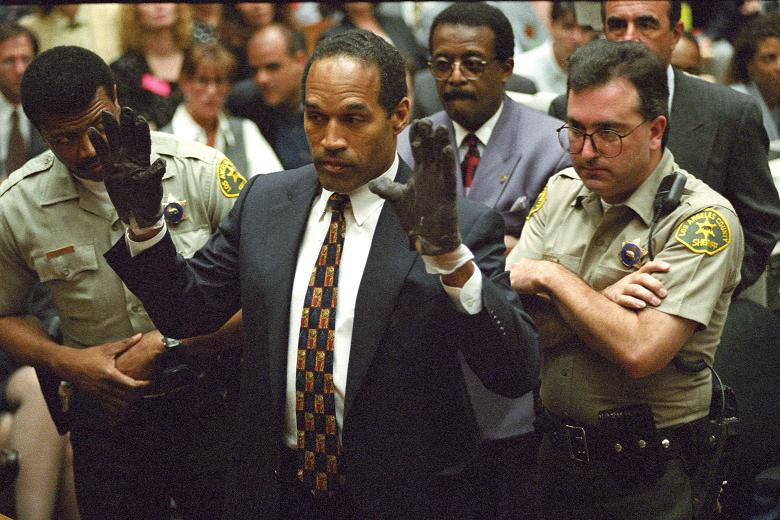
\includegraphics[height=5cm]{../images/OJSimpson.jpg}
\end{center}
\end{frame}




\subsection[]{The Western legal system}
\begin{frame}[fragile]{The Western legal system}

In a legal court case, the defendent is either innocent (not guilty) or guilty. But unless the defendent pleads guilty, we never know what the truth is. In fact, even if the defendent pleads guilty, there may be more going on!

\vspace{.5cm}
Our modern Western legal system is based on the principle of being ‘innocent until proven guilty’ or ‘proof beyond a reasonable doubt’.  \\
Hence we assume $H_{0}$: defendent is innocent. \\
Unless there is strong evidence for $H_{1}$: defendent is guilty.

\vspace{.5cm}
{\bf What the pros and cons of this type of legal system?}

\end{frame}

\begin{frame}[fragile]{}

In any legal case, there are 4 possible outcomes:  \\

{\small \begin{tabular}{|l|l|l|} \hline
 & Truth: $H_{0}$ is true  & Truth: $H_{0}$ is false \\ \hline
Decision: Retain $H_{0}$ & Acquit innocent person & Acquit guilty person. \\
& & (Type II error) \\ \hline
Decision: Reject $H_{0}$ & Convict innocent person & Convict guilty person. \\
& (Type I error) & \\ \hline
\end{tabular}}

\vspace{.5cm}
We can generalise this terminology, where $\alpha$ and $\beta$ are probabilities:  \\

{\small \begin{tabular}{|l|l|l|} \hline
 & Truth: $H_{0}$ is true  & Truth: $H_{0}$ is false \\ \hline
Decision: Retain $H_{0}$ & Specificity = $1-\alpha$ & False negative = $\beta$ \\
& & (Type II error) \\ \hline
Decision: Reject $H_{0}$ & False positive = $\alpha$ & Power or sensitivity = $1-\beta$ \\
& (Type I error) & \\ \hline
\end{tabular}}

\vspace{.5cm}
We set the Type I error to be small, typically $\alpha = 0.05$ (which is called the `signicance level'). Ideally we want the Power to be large.
\href{http://www.ncbi.nlm.nih.gov/pmc/articles/PMC2996198/}{\beamergotobutton{Article}}
\end{frame}

\begin{frame}[fragile]{}

Other contexts:  \\

{\small \begin{tabular}{|l|l|l|} \hline
Context & Type I error & Type II error \\ \hline
$H_{0}$: Patient is healthy & Wrong diagnosis & Undiagnosed condition \\
$H_{1}$: Patient has Diabetes & \href{https://canceraustralia.gov.au/publications-and-resources/position-statements/overdiagnosis-mammographic-screening}{\beamergotobutton{Breast Cancer}}
& \\ \hline
$H_{0}$: iPhone works & Wastage for Apple & Ruins Apple reputation \\ 
$H_{1}$: iPhone is faulty & &  \\ \hline
\end{tabular}}
\end{frame}


\subsection[]{Framework for Hypothesis Testing}
\begin{frame}[fragile]{Framework for Hypothesis Testing}

For each Hypothesis Test,  we use the following framework: \\

\vspace{.5cm}
\framebox{H} Set up the two hypotheses: $H_{0}$ and $H_{1}$. \\

\framebox{A} State the assumption(s) of the test, and justify whether they are valid from the sample.

\framebox{T} 
\begin{itemize}
\item State the Test Statistic, and it's distribution assuming $H_{0}$ is true. 
\item State what values argue against $H_{0}$.
\item Find the observed value of the Test Statistic.
\end{itemize}

\framebox{P} Calculate the $P$-value, which represents the probability of observing this sample (or more extreme) assuming $H_{0}$ is true.

\framebox{C} Weigh up the conclusion, based on the size of the $P$-value.
\end{frame}

\subsection[]{Defining Terms}
\begin{frame}[fragile]{Defining Terms}

\framebox{H} \\

\begin{itemize}
\item 
The Null hypothesis $H_{0}$ is the default hypothesis: what we currently believe to be true. \\
\item
The Alternate hypothesis $H_{1}$ is a new claim about the population. \\
\item The hypotheses are commonly articulated in terms of the unknown population parameter. Eg $H_{0}: \mu = 5$.
\item If so, then the alternate hypothesis can take 2 forms: \\
1 sided ($H_{1}: \mu > 5$ or
$H_{1}: \mu < 5$) or 2-sided ($H_{1}: \mu \neq 5$).
\item How to decide between a 1 or 2 sided test?
The decision must not be influenced by the data (`data snooping') – we must specify the hypotheses before we do the actual test. Hence, we always use a 2 sided test, unless we have prior evidence (eg a previous report) which suggests a 1 sided test.
\end{itemize}
\end{frame}


\begin{frame}[fragile]{}

\framebox{A} \\
The assumptions are necessary for the test to be valid. We check whether they appear valid from the sample. \\

\vspace{.5cm}
\framebox{T} \\
\begin{itemize}
\item The Test Statistic $\tau$ is a random variable, with a distribution which depends on the unknown parameter.
\item The observed value of the Test Statistic $\tau_{obs}$ (or $\tau_{0}$) is calculated from the sample.
\item Look at the distribution of $\tau$ to determine what values will argue against $H_0$ for $H_1$.
\item Hypothesis testing involves some theory about the random variable $\tau$ where every possible value $\{ \tau_{0} \}$ counts as some evidence about $H_{0}$. The Hypothesis Test weighs up  the evidence against $H_{0}$ based on the observed value.
\end{itemize}
\end{frame}

\begin{frame}[fragile]{}

\framebox{P} \\
\begin{itemize}
\item The $P$-value is the probability of observing $\tau_{0}$ or something more extreme (or unusual) under $H_{0}$. 

\item A small $P$-value either means that $H_{0}$ is true but the sample is highly rare, or that $H_{0}$ is false.

\item  The smaller the $P$-value, the stronger the evidence against $H_{0}$ for $H_{1}$.  

\item A large $P$-value means that the sample is consistent with $H_{0}$.

\item The critical region is the set of $\tau$ such that $H_{0}$ would be rejected.
\end{itemize}

\begin{tabular}{|l|l|l|} \hline
$P$-value & Correct language & Unhelpful Language \\ \hline
Small & Evidence against $H_{0}$ & $H_{0}$ is false or $H_{1}$ is true. \\
& Reject $H_{0}$  for $H_{1}$ & \\ \hline
Large & Data are consistent with $H_{0}$   & $H_{0}$ is true or $H_{1}$ is false. \\
& Retain $H_{0}$ & \\ \hline
\end{tabular}

\end{frame}

\begin{frame}[fragile]{}

\framebox{C} \\

‘The (null hypothesis) is ... never proved or established, but is possibly disproved, in the context of experimentation. Every experiment may be said to exist only in order to give the facts a chance of disproving the null hypothesis.’ (Ronald Fisher, Design of Experiments, 1935, p19).

\begin{itemize}
\item There is no final proof that $H_{0}$ is true or false.

\item The conclusion is not `Accept' $H_{0}$ or $H_{1}$, as  we have assumed $H_{0}$ to be true. 
That is, we have not proved $H_{0}$ true, rather we look for evidence about whether it is false.

\item  If the $P$-value is small, it suggests there is evidence against  $H_{0}$. If the $P$-value is not small, then it suggests the data are consistent with $H_{0}$

\item By `small', a common convention is $\alpha = 0.05$. That is, for $P$-values under 0.05, we suggest there is evidence against  $H_{0}$.
\end{itemize}
\end{frame}

\begin{frame}{}

\begin{center}
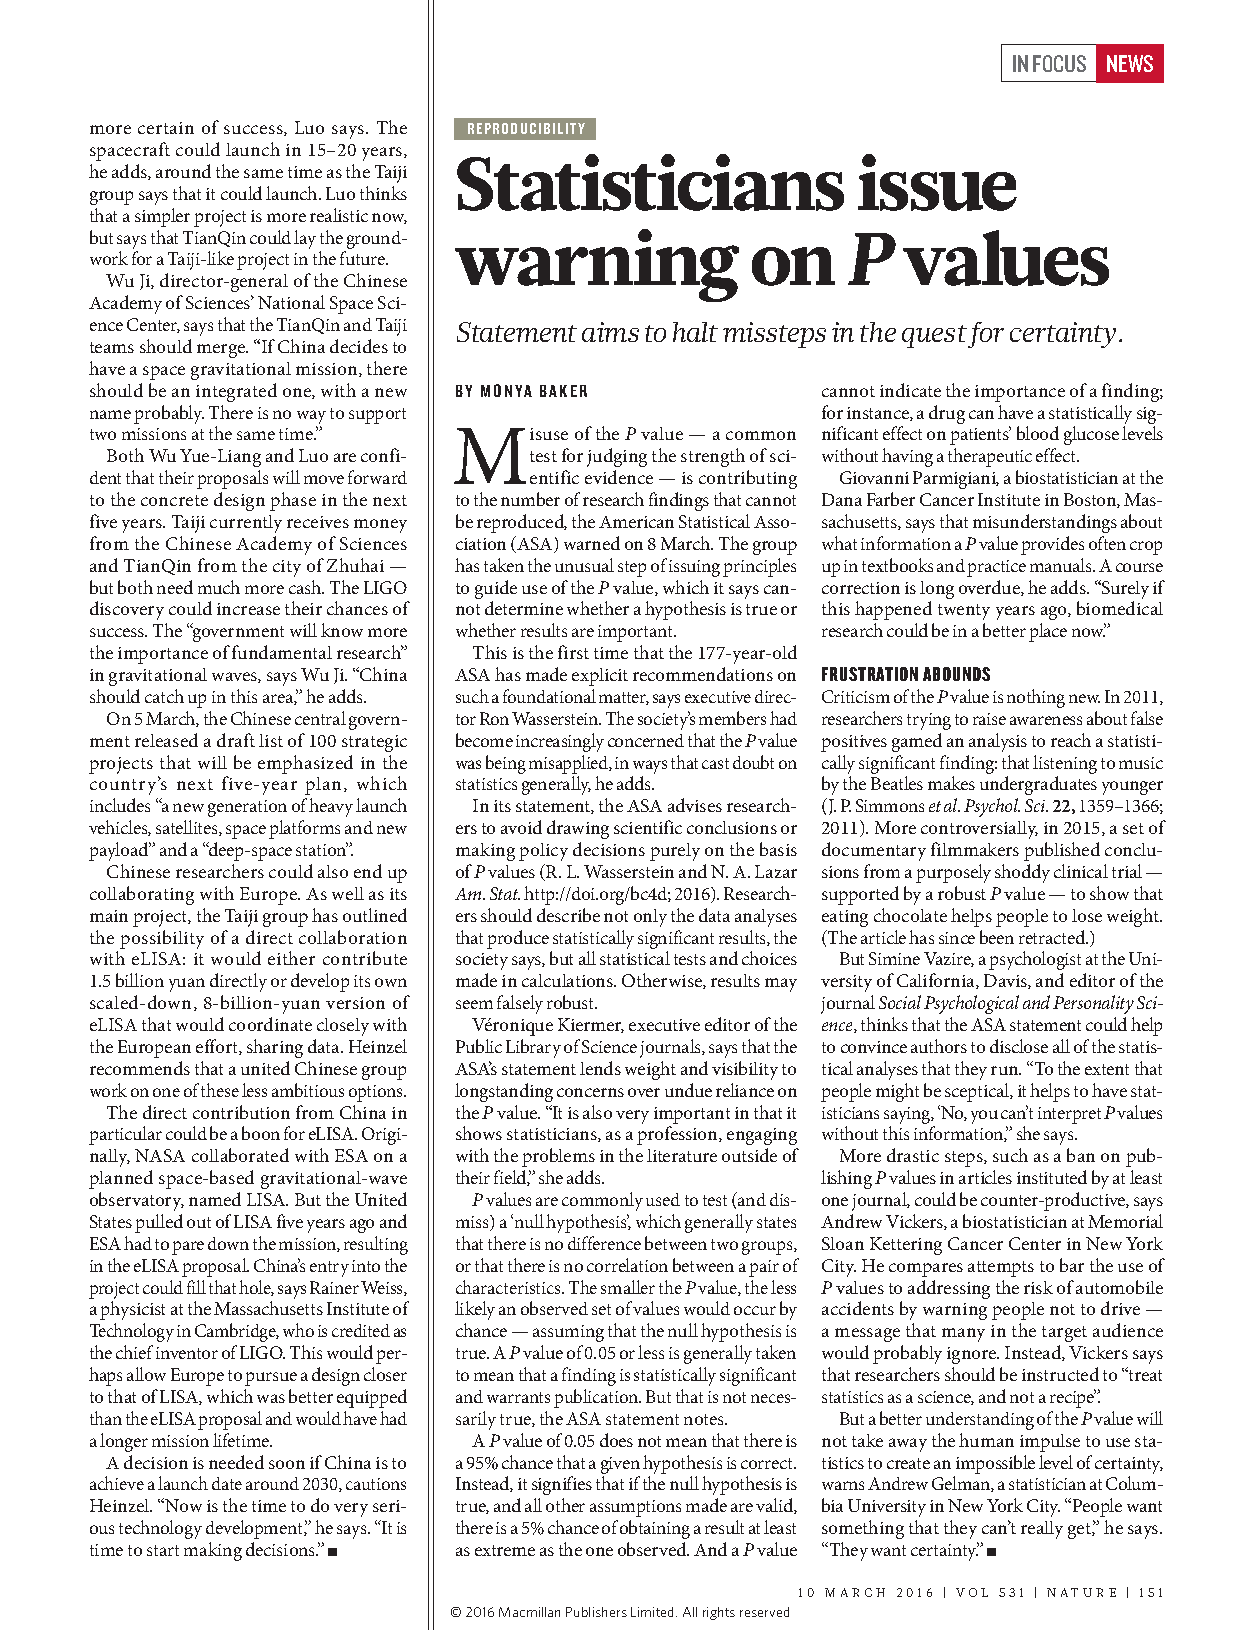
\includegraphics[height=11cm]{../images/PvaluesNature2016.pdf}
\end{center}
\end{frame}

\end{document}
